\PassOptionsToPackage{xetex}{xcolor}
\PassOptionsToPackage{xetex}{graphicx}
\documentclass[a4paper,landscape,headrule,footrule,xetex]{foils}

%%
%%%  Macros
%%%
\newcommand{\logo}{~}
\MyLogo{HG2052 (2020)}
%\newcommand{\Story}{\SHA{HOUN}{The Hound of the Baskervilles}}

\newcommand{\header}[3]{%
\title{\vspace*{-2ex} \Large HG2052
\\\large  Language, Technology and the Internet
\\[2ex] \Large  \emp{#2}}
\author{\blu{Francis Bond}   \\ 
\normalsize  \textbf{Division of Linguistics and Multilingual Studies}\\
\normalsize  \url{http://www3.ntu.edu.sg/home/fcbond/}\\
\normalsize  \texttt{bond@ieee.org}}
\MyLogo{HG2052 (2020)}
\date{#1}
\renewcommand{\logo}{#2}
 \hypersetup{
   pdfinfo={
     Author={Francis Bond},
     Title={#1: #2},
     Subject={HG2052: Language, Technology and the Internet},
     Keywords={Language, Technology, Internet},
     License={CC BY 4.0}
   }
 %  pdfcopyright={Copyright © Francis Bond. Creative Commons 4.0 Attribution License.}
 %  pdflicenseurl={http://creativecommons.org/licenses/by/4.0/}
 }
}


%%
%% Multilingual Stuff
%%
\usepackage[a4paper,landscape,margin=25mm]{geometry}

\usepackage{fontenc}
\usepackage{polyglossia}
\setmainlanguage{english}
\setmainfont{TeX Gyre Pagella}
%\setmainfont{Linux Libertine}
%\setmainfont{Charis SIL}
\newfontfamily{\ipafont}{Gentium}
\newcommand{\ipa}[1]{{\ipafont\selectfont #1}}
\usepackage{xeCJK}

\setCJKmainfont{Noto Sans CJK SC}
\setCJKsansfont{Noto Sans CJK SC}
%\setCJKttfont{Noto Sans CJK SC}
%\setCJKmainfont{WenQuanYi Micro Hei}
%\clearpage
%\setCJKmainfont{AR PL SungtiL GB}

\usepackage[xetex]{xcolor}
\usepackage[xetex]{graphicx}
\newcommand{\blu}[1]{\textcolor{blue}{#1}}
\newcommand{\grn}[1]{\textcolor{green}{#1}}
\newcommand{\hide}[1]{\textcolor{white}{#1}}
\newcommand{\emp}[1]{\textcolor{red}{#1}}
\newcommand{\txx}[1]{\textbf{\textcolor{blue}{#1}}}
\newcommand{\lex}[1]{\textbf{\mtcitestyle{#1}}}

\usepackage{pifont}
\renewcommand{\labelitemi}{\textcolor{violet}{\ding{227}}}
\renewcommand{\labelitemii}{\textcolor{purple}{\ding{226}}}

\newcommand{\subhead}[1]{\noindent\textbf{#1}\\[5mm]}

\newcommand{\Bad}{\emp{\raisebox{0.15ex}{\ensuremath{\mathbf{\otimes}}}}}
\newcommand{\bad}{*}

\newcommand{\com}[1]{\hfill \textnormal{(\emp{#1})}}%
\newcommand{\cxm}[1]{\hfill \textnormal{(\txx{#1})}}%
\newcommand{\cmm}[1]{\hfill \textnormal{(#1)}}%
\usepackage{amssymb}
\usepackage{relsize,xspace}
\newcommand{\into}{\ensuremath{\rightarrow}\xspace}
\newcommand{\ent}{\ensuremath{\Rightarrow}\xspace}
\newcommand{\nent}{\ensuremath{\not\Rightarrow}\xspace}
\newcommand{\tot}{\ensuremath{\leftrightarrow}\xspace}
\usepackage{url}
\usepackage[hidelinks]{hyperref}
\hypersetup{
     colorlinks,
     linkcolor={blue!50!black},
     citecolor={red!50!black},
     urlcolor={blue!80!black}
}
%\usepackage{hyperxmp}
\usepackage{url}
\newcommand{\lurl}[1]{\MyLogo{\url{#1}}}

\usepackage{mygb4e}
\let\eachwordone=\itshape
\newcommand{\lx}[1]{\textbf{\textit{#1}}}
\newcommand{\ix}{\ex\it}

\newcommand{\cen}[2]{\multicolumn{#1}{c}{#2}}
%\usepackage{times}
%\usepackage{nttfoilhead}
\newcommand{\myslide}[1]{%
\foilhead[-25mm]{\raisebox{12mm}[0mm]{\emp{#1}}}%
\leftheader{}%
\MyLogo{\logo}}

\newcommand{\mytask}[1]{%
\foilhead[-25mm]{\raisebox{12mm}[0mm]{\emp{#1}}}
\leftheader{🔍 Hi}%
\MyLogo{\logo}}

\newcommand{\myslider}[1]{\rotatefoilhead[-25mm]{\raisebox{12mm}[0mm]{\emp{#1}}}}
%\newcommand{\myslider}[1]{\rotatefoilhead{\raisebox{-8mm}{\emp{#1}}}}

\newcommand{\section}[1]{\myslide{}{\begin{center}\Huge \emp{#1}\end{center}}}

\usepackage{tcolorbox}
% \newcommand{\task}{\marginpar{\raisebox{-1ex}{\large
%       \tcbox[colframe=red,colback=white,arc=3pt]{\textbf{?}}}}}
% \newcommand{\task}{\marginpar{\raisebox{-1ex}{
%       \hspace{-0.5em}\tcbox[colframe=red,colback=white,arc=3pt]{%
%         \includegraphics[width=1.5em]{pics/detective}}}}}
\newcommand{\task}{\marginpar{\raisebox{-2ex}{
      \hspace{-0.5em}\reflectbox{\includegraphics[width=2em]{pics/detective}}}}}

\usepackage[lyons,j,e,k]{mtg2e}
\renewcommand{\mtcitestyle}[1]{\textcolor{teal}{\textsl{#1}}}
%\renewcommand{\mtcitestyle}[1]{\textsl{#1}}
\newcommand{\chn}{\mtciteform}
\newcommand{\cmn}{\mtciteform}
\newcommand{\iz}[1]{\textup{\texttt{\textcolor{blue}{\textbf{#1}}}}}
\newcommand{\con}[1]{\textsc{#1}}
\newcommand{\gm}{\textsc}
\newcommand{\cmp}[1]{{[\textsc{#1}]}}
\newcommand{\sr}[1]{\ensuremath{\langle}#1\ensuremath{\rangle}}
\usepackage[normalem]{ulem}
\newcommand{\ul}{\uline}
\newcommand{\uul}{\uuline}
\newcommand{\wl}{\uwave}
\newcommand{\vs}{\ensuremath{\Leftrightarrow}~}
%%%
%%% Bibliography
%%%
\usepackage{natbib}
%\usepackage{url}
\usepackage{bibentry}


%%% From Tim
\newcommand{\WMngram}[1][]{$n$-gram#1\xspace}
\newcommand{\infers}{$\rightarrow$\xspace}



\usepackage{rtrees,qtree}
\renewcommand{\lf}[1]{\br{#1}{}}
\usepackage{avm}
%\avmoptions{topleft,center}
\newcommand{\ft}[1]{\textsc{#1}}
\newcommand{\val}[1]{\textit{#1}}
\newcommand{\typ}[1]{\textit{#1}}
\avmfont{\sc}
%\avmvalfont{\sc}
\renewcommand{\avmtreefont}{\sc}
\avmsortfont{\it}


%%% From CSLI book
\newcommand{\mc}{\multicolumn}
\newcommand{\HD}{\textbf{H}\xspace}
\newcommand{\el}{\< \>}
\makeatother
\long\def\smalltree#1{\leavevmode{\def\\{\cr\noalign{\vskip12pt}}%
\def\mc##1##2{\multispan{##1}{\hfil##2\hfil}}%
\tabskip=1em%
\hbox{\vtop{\halign{&\hfil##\hfil\cr
#1\crcr}}}}}
\makeatletter

\newcommand{\sh}[1]{\href{https://www.arthur-conan-doyle.com/index.php?title=#1}{#1}}
\newcommand{\SHA}[2]{\href{https://www.arthur-conan-doyle.com/index.php?title=#1}{\textit{#2}}}


\header{Lecture 8}{Text and Meta-Text}





\begin{document}
\bibliographystyle{apalike}
\nobibliography{abb,mtg,nlp,ling}

\maketitle


\myslide{Text and Meta-text}
\MyLogo{and Zombies}
\begin{itemize}
\item Revision of Web As Corpus
\item Explicit Meta-data
  \begin{itemize}
  \item Keywords and Categories
  \item Rankings
  \item Structural Markup
  \end{itemize}
\item Implicit Meta-data
  \begin{itemize}
  \item Links and Citations
  \item Tags
  \item Tables
  \item File Names
  \item Translations
  \end{itemize}
\end{itemize}



\myslide{Revision of the Web as Corpus}
\begin{itemize}
\item \blu{Direct Query}: Search Engine as Query tool and WWW as corpus?
\\  (Objection: Results are not reliable)
\begin{itemize}
\item Population and exact hit counts are unknown → no statistics
possible.
\item Indexing does not allow to draw conclusions on the data.
\item[\Bad] Google is missing functionalities that linguists /
lexicographers would like to have.
\end{itemize}
\item \blu{Web Sample}: Use search engine to download data from the
net and build a corpus from it.
\begin{itemize}
\item known size and exact hit counts → statistics possible.
\item people can draw conclusions over the included text types.
\item (limited) control over the content.
\item[\Bad] sparser data
\end{itemize}
\end{itemize}

\myslide{Direct Query}
\begin{itemize}
\item Accessible through search engines (Google API, Yahoo API, Scripts)

\item Document counts are shown to correlate directly with ``real''
  frequencies (Keller 2003), so search engines can help - but...
  \begin{itemize}
  \item lots of repetitions of the same text (not representative)
  \item very limited query precision (no upper/lower case, no punctuation...)
  \item only estimated counts, often hard to reproduce exactly
  \item different queries give wildly different numbers
  \end{itemize}
\end{itemize}

\myslide{Web Sample}
\MyLogo{}
\begin{itemize}
\item Extracting and filtering web documents to create linguistically
  annotated corpora (Kilgarriff 2006)
  \begin{itemize}
  \item gather documents for different topics (balance!)
  \item exclude documents which cannot be preprocessed with available
    tools (here taggers and lemmatizers)
  \item exclude documents which seem irrelevant for a corpus (too short or
    too long, word lists,...)
  \item do this for several languages and make the corpora available
  \end{itemize}
\end{itemize}


\myslide{Internet Corpora: Outline}
\MyLogo{\url{http://corpus.leeds.ac.uk/internet.html}}

\begin{enumerate}
\item Select Seed Words (500)
\item Combine to form multiple queries (6,000)
\item Query a search engine and retrieve the URLs (50,000)
\item Download the files from the URLS (100,000,000 words)
\item Postprocess the data (encoding; cleanup; tagging and parsing)
\end{enumerate}

Sharoff, S (2006) Creating general-purpose corpora using automated search engine queries. In M. Baroni, S. Bernardini (eds.) WaCky! Working papers on the Web as Corpus, Bologna, 2006.

\myslide{Internet Corpora Summary}
\MyLogo{}
 
\begin{itemize}
\item The web can be used as a corpus
  \begin{itemize}
  \item Direct access
    \begin{itemize}
    \item Fast and convenient
    \item Huge amounts of data
    \item[\Bad] unreliable counts 
    \end{itemize}
  \item Web sample
    \begin{itemize}
    \item Control over the sample
    \item Some setup costs (semi-automated)
    \item[\Bad] Less data 
    \end{itemize}
  \end{itemize}
\item Richer data than a compiled corpus
\item[\Bad] Less balanced, less markup
\end{itemize}


\myslide{Explicit Metadata}
\MyLogo{}
\begin{itemize}
\item You can get information from metadata within documents
  \begin{itemize}
  \item When they are accurate they are very good
  \item They are often inaccurate
    \begin{itemize}
    \item Sometimes deliberately deceitful
    \item More often incomplete or out-of-date
    \end{itemize}
  \end{itemize}
      \begin{quote} \itshape
    Never attribute to malice that which is adequately explained by stupidity.

     \end{quote} %%% FIXME attribute
      \begin{flushright}
               Hanlon's Razor
      \end{flushright}
      \begin{quote} \itshape
        You have attributed conditions to villainy 
        that simply result from stupidity
      \end{quote}
       \begin{flushright}
         Robert A. Heinlein (1941) \textit{Logic of Empire}
       \end{flushright}
\end{itemize}

\myslide{HTML Metadata}
\MyLogo{}
\begin{itemize}
\item Most document types contain metadata of some description:
  \begin{quote}
    \smaller[2]
\begin{verbatim}
  <head>
    <title>CSLI LinGO Lab</title>
    <META HTTP-EQUIV="Content-Type" CONTENT="text/html; charset=iso-8859-1">
    <meta http-equiv="Content-Style-Type" content="text/css">
    <meta name="keywords" content="linguistic grammars online, 
     LinGO, computational linguistics,
     head-driven phrase structure grammar, hpsg, natural language processing,
     parsing, generation, augmentative and alternative communication, aac,
     LinGO Redwoods, multiword expressions, MWE, grammar matrix">
    <meta name="description" content="This page provides information about
     the CSLI Linguistic Grammars Online (LinGO) Lab at Stanford
     University.">
\end{verbatim}
  \end{quote}
\item Should we also extract out this data, or is metadata too
  unreliable to consider using?
\end{itemize}

\myslide{PDF Metadata}

\begin{itemize}
\item Checkout this file (now look at earlier weeks)
  \begin{small}
\begin{verbatim}
InfoKey: Creator
InfoValue: xetex(k) 5.98 Copyright 2009 Radical Eye Software
InfoKey: Title
InfoValue: Lecture 11:Text and Meta-Text
InfoKey: Author
InfoValue: Francis Bond
InfoKey: Producer
InfoValue: GPL Ghostscript 8.71
InfoKey: Keywords
InfoValue: Language, Technology, Internet
InfoKey: Subject
InfoValue: HG2052/HG252: Language, Technology and the Internet
InfoKey: ModDate
InfoValue: D:20120315121040+08'00'
InfoKey: CreationDate
InfoValue: D:20120315121040+08'00'
PdfID0: 39bb293fa576c18e1ae64480cb8974
PdfID1: 39bb293fa576c18e1ae64480cb8974
NumberOfPages: 23
\end{verbatim}
  \end{small}
\end{itemize}

\myslide{HTML Metadata}
\MyLogo{\url{http://www.yourhtmlsource.com/promotion/metatags.html}}
\begin{itemize}
\item HTML Metadata is generally considered unreliable
  \begin{itemize}
  \item Authors don't see it, so they don't update it
  \item As it is unseen, it is easy to lie in the MetaData
  \end{itemize}
\end{itemize}
\begin{quotation} \small 
  It wasn't long before webmasters with no scruples saw an opportunity to gain favour with the search engines by adding in keywords that did not pertain to the content of their pages. Various tactics were thought up to get ranked higher for certain keywords, and an entire industry sprang up to optimise search engine positioning. This was, in effect, cheating, and ``keyword spamming'' became a serious problem for search engines, who vainly attempted to add filters that would notice when a webmaster was loading up on the wrong keywords.
\end{quotation}



\myslide{Keywords and Categories}
\begin{itemize}
\item Sites with \emp{visible tags} are more trustworthy/reliable
\item Tags within blogs/photo cites
\item Keywords in journals and conferences
\end{itemize}

\myslide{Example tags from Science Professor}
\MyLogo{\url{http://science-professor.blogspot.com/}}
\begin{verbatim}
# academia (109)
# academic novels (9)
# accounting nightmares (10)
# administrative assistants (7)
# adviser-student (69)
# attempt at humor (18)
# awards (7)
# bizarre (56)
# blogging (22)
# books (23)
# broader impacts (8)
# career issues (27)
# cats (19)
# citations and citation index (19) 
\end{verbatim}


\myslide{Rankings}
\MyLogo{}

\begin{itemize}
\item Another good source of meta-data is rankings/forums
  \begin{description}
  \item[HG251] ★★★★
  \item[Q A] Solved
  \end{description}
\item \blu{Sentiment Analysis} tries to judge whether text is favorable or unfavorable
  \begin{itemize}
  \item Link text to rankings for data
  \item Link posts to tags for usefulness in QA
  \end{itemize}
\end{itemize}

\myslide{hungry\,go\,where}

\begin{verbatim}
Overall: 7  Recommend.
I spent about S$10 Per Person

    Food/Beverage: 6
    Ambience: 5
    Value: 9
    Service: 5

Cheap but not very cheerful                     10 June, 2010 
\end{verbatim}

\begin{small}
  Absolutely love this neighbourhood eatery, mainly because I have
  been eating here since I was a child, so it brings back many happy
  memories. Granted, service is kind of lacking but a cheap and yummy
  home-style meal can always be had. Must-haves for me are the Honey
  Pork (love the 3 or 4 little green peas they garnish it with), Ayam
  Buah Keluak, Bakwan Kepeting (meatball soup) and Sayur Lodeh. The
  Otak and Ngor Hiang are not bad too.
\end{small}


% \myslide{Structural Markup}
\myslide{Links and Citations}

\begin{itemize}
\item Citation frequency can be used to measure
  the \blu{impact} of an article.
\begin{itemize}
\item Simplest measure: Each article gets one vote -- not
  very accurate.
\end{itemize}
\item On the web: citation frequency = \blu{inlink count}
\begin{itemize}
\item A high inlink count does not necessarily
  mean high quality \ldots
\item \ldots mainly because of link spam.
\end{itemize}
\item Better measure: \blu{weighted} citation frequency or citation rank
\begin{itemize}
\item An article's vote is weighted according to its
  citation impact. 
\item This  can be formalized in a   well-defined way and calculated.
\end{itemize}
\end{itemize}

 \myslide{Structure}

 \begin{itemize}
 \item Structural Markup gives useful cues
   \begin{itemize}
   \item Words in headers are often good keywords
   \item TableOfContents!
\begin{verbatim}
1 Review
1.1 Language Identification
1.2 Normalization
2 Text and Meta-text
2.1 Implicit Tags
2.1 Explicit Tags
\end{verbatim}
   \end{itemize}


 \end{itemize}


\myslide{Implicit Metadata}
\begin{itemize}
\item You can get clues from metadata within documents
  \begin{itemize}
  \item as they are non-intended, they tend to be noisy
  \item but they are rarely deceitful
  \end{itemize}
\end{itemize}


 \myslide{Tags}
\MyLogo{\url{http://aclweb.org/anthology-new/P/P10/P10-1130.pdf}}

\begin{itemize}
\item Hypertext Anchors and other formatting gives phrase boundaries
\begin{verbatim}
whereas McCain is secure on the topic, Obama
<a>[VP worries about winning the pro-Israel vote]</a>

[NP [NP Libyan ruler]
<a>[NP Mu‘ammar al-Qaddafi]</a>] referred to
\end{verbatim}
  Mainly NPs 
\item This can be very useful in restricting parser possibilities
\end{itemize}


Valentin I. Spitkovsky, Daniel Jurafsky, Hiyan Alshawi (2010) \textit{Profiting from Mark-Up: Hyper-Text Annotations for Guided Parsing} ACL


 \myslide{Tables}
\MyLogo{}
 \begin{itemize}
 \item You can learn many things from Tables
   \begin{itemize}
   \item for example, categories
   \end{itemize}
   \begin{tabular}{lrlll}
     \textbf{Vehicle} & \textbf{Price} & \textbf{Manufacturer} & \textbf{Type} & \textbf{Rating} \\
     \hline
     Raum & XXX & Toyota & Hatch-back & Solid \\
     icw30 & XXX & Hyundae & Station Wagon & Exciting \\
     Corolla & XXX & Toyota & Station Wagon & Solid \\
     Camry & XXX & Toyota & Sedan & Bland
   \end{tabular}
   \\[3ex] Toyota $\subset$ manufacturer
 \end{itemize}

 \myslide{File Names}
 \begin{itemize}
 \item How to find definitions?
   \begin{itemize}
   \item Look for files called \url{glossary}, \url{dictionary}, \ldots
   \end{itemize}
 \item Is there an English version of this?
   \begin{itemize}
   \item \url{http://nlpwww.nict.go.jp/wn-ja/index.ja.html}
   \item \url{http://nlpwww.nict.go.jp/wn-ja/index.en.html}
   \end{itemize}
 \end{itemize}

 \myslide{Translations}

 \begin{itemize}
 \item A translation into another language can be seen as markup
 \end{itemize}

\myslide{Bracketed Glosses}
\CJKfamily{gbsn}
\begin{verbatim}
GPS	
通用④回解诀者
28附录:(通用④回解诀者》(GPS)计算机程序解决・・河内塔。
{2069:corpus0.txt}

SomeThoughtsConcerningEducation	
教育漫话
笔者在认真阅读洛克的教育著作《教育漫话》
(SomeThoughtsConcerningEducation)、
《关于理解的指导》以及《贫穷儿童劳动学校计划》
(PlanofWorkingSchoolforPoor ...
{25094:corpus0.txt}
\end{verbatim}
\CJKfamily{min}

\myslide{Cross-lingual Disambiguation}

\begin{exe}
  \ex \eng{I$_1$ saw$_2$ the kid$_3$ with a telescope$_4$}
  \ex \glll Φ$_1$ 望遠鏡$_4$ で 子供$_1$ を 見た$_2$ \\
  {} bouenkyou de kodomo wo mita \\
 NULL telescope with child \textsc{acc} see-past \\
 \trans With the telescope, I saw the kid.
\end{exe}
\begin{itemize}
\item We can disambiguate the PP attachment: \lex{de} only modifies verbs
\item We can disambiguate the verb \lex{see/saw}: \lex{mita} is only ``see''
\item We can resolve the zero pronoun: It must be the speaker. 
\end{itemize}

\myslide{Query Data}
AOL user 2708:
\begin{itemize}\addtolength{\itemsep}{-1ex}
\item revenge tactics
\item the woman's book of revenge
\item dirty tricks for chicks
\item \ldots
\item locatecell.com
\item what can i do to an old lover for revenge
\item mean revenge tactics
\item death records in hampstead
\end{itemize}

\myslide{Wikipedia Redirections}
\MyLogo{http://en.wikipedia.org/wiki/Wikipedia:Redirect}

\begin{itemize}\addtolength{\itemsep}{-1ex}
\item  Alternative names (\eng{Edison Arantes do Nascimento} \into \eng{Pelé}).
\item Abbreviations (\eng{DSM-IV} \into \eng{Diagnostic and Statistical Manual of Mental Disorders}).
\item Alternative spellings or punctuation. (\eng{Colour} \into \eng{Color}; \eng{Al-Jazeera} \into \eng{Al Jazeera}).
\item Likely misspellings (\eng{Condoleeza Rice} \into \eng{Condoleezza Rice}).
\item Plurals (\eng{Greenhouse gases} \into \eng{Greenhouse gas}).
\item Related words (\eng{Symbiont} \into \eng{Symbiosis}).
\item Representations using ASCII characters (\eng{Kurt Goedel} and \eng{Kurt Godel} \into  \eng{Kurt Gödel}). 
 \end{itemize}

Unfortunately redirects are rarely typed (so we don't know the
relation, but have to infer it).
 
\myslide{Cross Wikipedia Links}
\MyLogo{}
\begin{description}\addtolength{\itemsep}{-1ex}
\item[en] Forensic linguistics
%\item[bg] Криминоложка лингвистика
\item[ca] Lingüística forense
\item[cs] Forenzní lingvistika
\item[de] Forensische Linguistik
\item[es] Lingüística forense
\item[nl] Forensische taalkunde
\item[no] Forensisk lingvistikk
\item[tr] Adlî dil bilimi
\item[zh] 司法语言学
\end{description}

\myslide{Deliberate Deceit: Phishing}
\MyLogo{\url{http://en.wikipedia.org/wiki/Phishing}}
\begin{itemize}
\item \blu{Phishing} is a way of attempting to acquire information
  such as usernames, passwords, and credit card details by
  masquerading as a trustworthy entity in an electronic communication.
\item Communications typically pretend to be from social web sites, auction sites, online payment processors or IT administrators.
\item Phishing is typically carried out by e-mail spoofing, linking
  users to a fake website whose look and feel are almost identical
  to the legitimate one.
\item Phishing is an example of social engineering.
\item A phishing technique was described in detail in 1987, and (according to its creator) the first recorded use of the term \textit{phishing} was made in 1995.
\end{itemize}

\myslide{From my own spam box}
\MyLogo{}
\begin{verbatim}
System Administrator s28407548@tuks.co.za via srs.ieee.org 
to undisclosed recipients

You have exceeded the storage limit on your mailbox.

You will not be able to send or receive new mail until 
you upgrade your email quota.

Click the below link and fill the form to upgrade your
 account.

http://millerofficetrailers.com/forms/use/hepldesk/form1.html

System Administrator
192.168.0.1
\end{verbatim}

\myslide{The fake form}
\begin{center}
  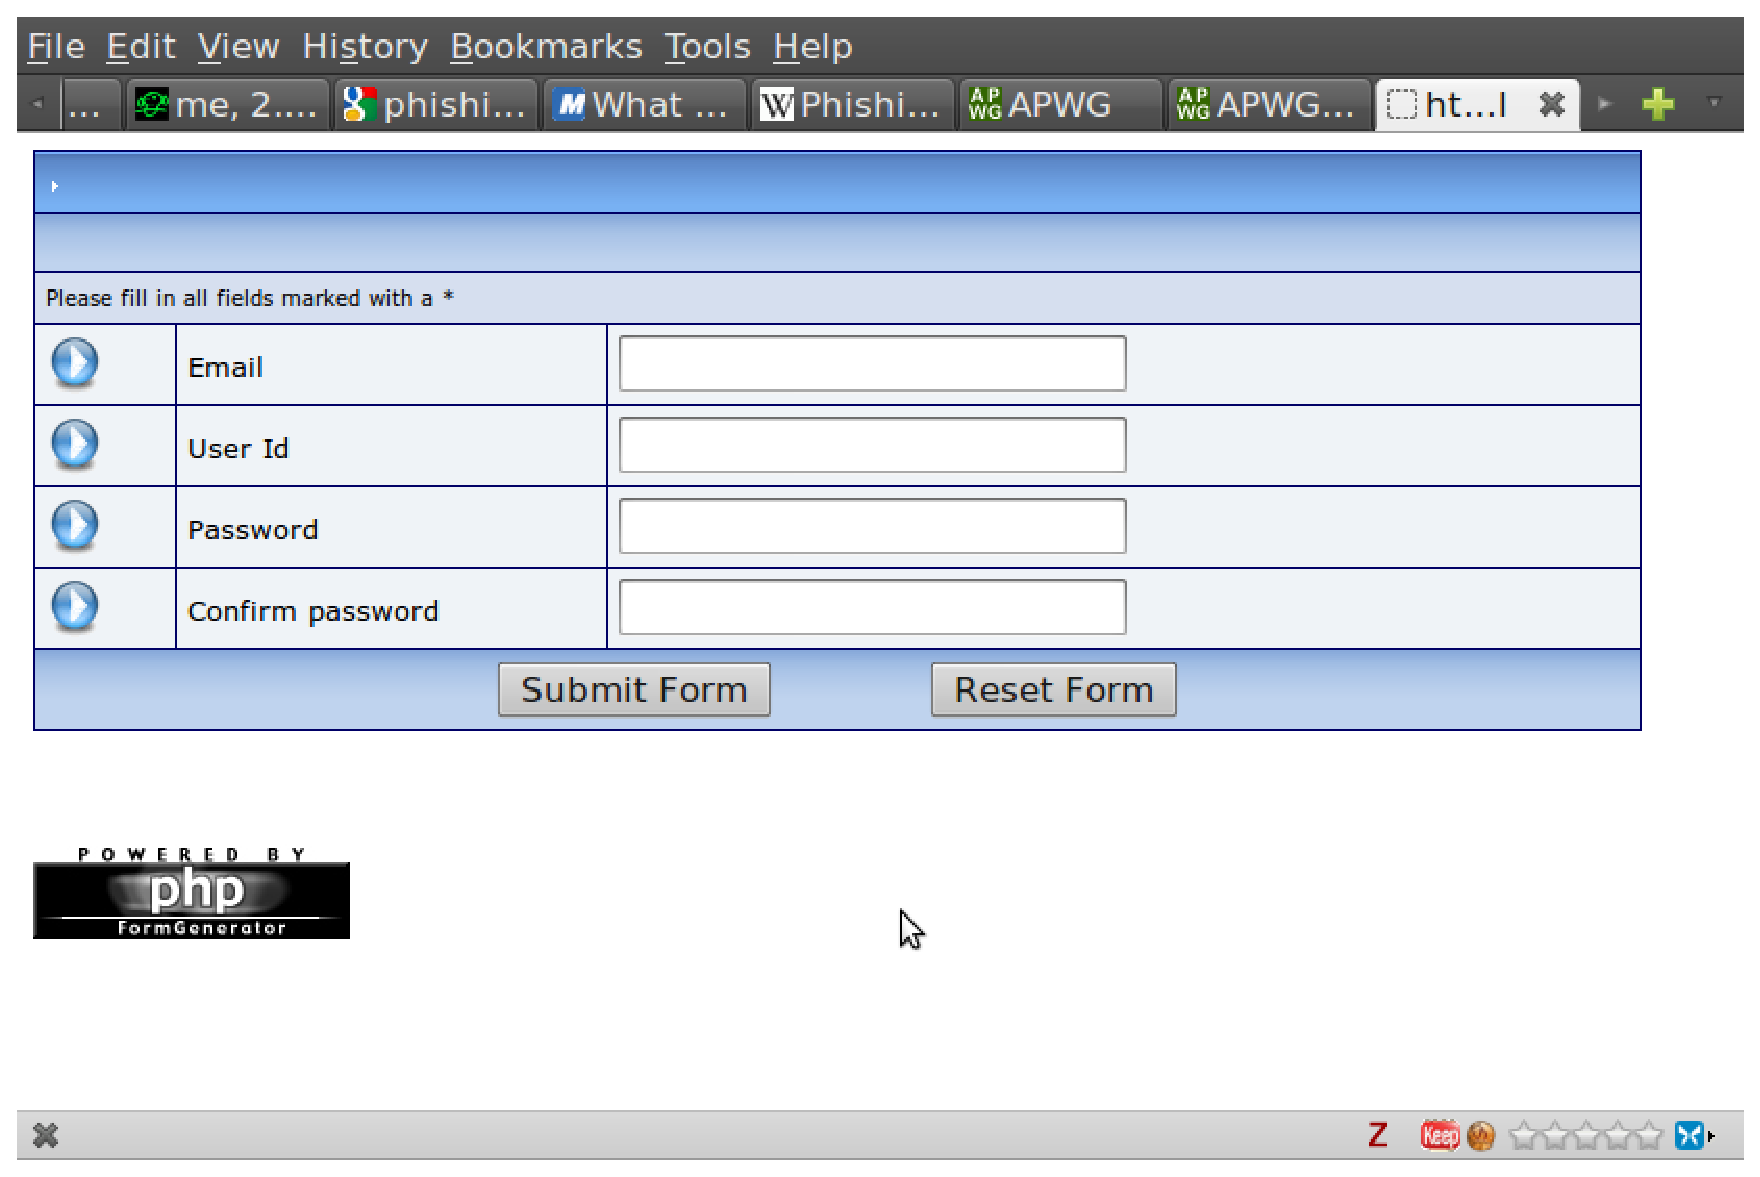
\includegraphics[width=0.8\textwidth]{../pics/phishing.eps}
\end{center}

\myslide{Some Distinguishing Features}

\begin{itemize}
\item Surprisingly many grammatical mistakes
\item Spoofed URLs
\item Ultimatums
\item Weird misspellings: \url{NTU.edu.org}
\end{itemize}




\myslide{Fake News}

\begin{itemize}
\item Fake news is \emp{false} news
  \begin{itemize}
  \item Malicously False News
  \item Satire
  \item Disinformation
  \item Misinformation
  \item Rumour
  \end{itemize}
\item Fake news is \emp{intentionally} and \emp{verifiably} false news
  \emp{published by a news outlet}
\end{itemize}

\myslide{Analyzing Language in Fake News}

\begin{itemize}
\item Verifying facts is difficult, but we can analyze language \citep{rashkin-etal-2017-truth}
  \\
  \begin{small}
    \begin{tabular}{lrll}
      Phenomenon & Ratio & Example & Type \\
      Swear& 7.00& Ms. Rand, who has been damned to eternal torment
                  ...& S\\
      2p (You) & 6.73 & You would instinctively justify \ldots & P  \\
      Modal Adv &2.63 &  ... investigation of Clinton  was inevitably
                        linked ... & S \\
      Negation &  1.51 &  There is nothing that outrages liberals more
                         than ...  & H \\
      Superlatives &   1.17 &  Fresh water is the single most
                              important natural resource  &  P \\
      \hline
      Comparitives &   0.86  &  ... from fossil fuels to
                               greener sources of energy  & P  \\
Hear & 0.50 & The prime minister also spoke about the commission ... &
                                                                       S \\
      Number & 0.43 &  ... 7 million foreign tourists coming to the
                      country in 2010 & S \\
    \end{tabular}
  \end{small}
  \begin{itemize}
  \item   Satire, Hoax, Propoganda vs real news
  \item Ratio of appearance in fake to real news
  \end{itemize}
\item We can identify things likely to be fake news just from the
  language
\item But the single most useful piece of evidence (feature) is the
  source --- where it comes from

\end{itemize}

\myslide{Why is this important?}
\MyLogo{}
\begin{itemize}
\item The 1990s started a revolution in empirical linguistics
  \begin{itemize}
  \item New insights come from \emp{Data Mining} large text collections
    \begin{itemize}
    \item Corpus Linguistics
    \item You can do with a computer what you can't do with paper
    \end{itemize}
  \item New tools come from supervised \emp{Machine Learning}
  \end{itemize}
\item Annotation is expensive and tedious to do
\item We want to get annotation for free
\item People appreciate clever ideas
\item In Singapore multiple-languages can serve as annotation, \ldots
\end{itemize}

% \myslide{Acknowledgments}

% \begin{itemize}
% \item Many slides from Tim Baldwin's \textit{Web as Data} 
%   \\ (Melbourne University 433-352)
% \item Excellent introduction to Information Retrieval, including web searching:
% \\ Christopher D. Manning, Prabhakar Raghavan and Hinrich Schütze, \textit{Introduction to Information Retrieval}, Cambridge University Press. 2008. 
% \\ \url{http://nlp.stanford.edu/IR-book/information-retrieval-book.html}
% \\ \textit{Determining the vocabulary of terms} deals with tokenization/normalization
% \end{itemize}
\end{document}



%%% Local Variables: 
%%% coding: utf-8
%%% mode: latex
%%% TeX-PDF-mode: t
%%% TeX-engine: xetex
%%% End: 
